\documentclass[a4paper,11pt]{report}
\usepackage[italian]{babel}
\usepackage[utf8]{inputenc}
\usepackage[total={170mm,267mm},top=15mm,bottom=15mm,left=21mm,right=21mm]{geometry}
\usepackage{graphicx}

\begin{document}

\begin{titlepage}
  \clearpage\thispagestyle{empty}
  \centering
  \vspace{1cm}
  {\normalsize Informatica - Area scientifica \\  Dipartimento di Scienze matematiche, informatiche e multimediali\\  Università di Udine \par}
  \vspace{3cm}
  {\Huge \textbf{Progetto di Social Computing}}\\
  \vspace{4cm}
  {\Large  Parata Loris (144338) \\ Arzon Francesco (142439)\\ Dal Fabbro Lorenzo (142300)\\ Galvan Matteo (142985) \\ }
  \vspace{12cm}
  {\normalsize Anno accademico 2020/2021}
  \pagebreak
\end{titlepage}

\tableofcontents{}
\pagebreak
\chapter{Sottografo di Twitter}
\section{Introduzione}
Il primo progetto di Social Computing consiste nello studio della rete sociale di 5 utenti di Twitter.\\
Lo studio è stato svolto mediante la costruzione di un grafo, rappresentante  rete sociale, costituto dai 5 utenti principali e della loro relativa rete di contatti costituita dai loro follower, following e da rispettivi sottoinsiemi campionati in maniera random.
In specifico abbiamo analizzato la relazione diretta di \textbf{follow} tra tutti i nodi del grafo ed i 5 profili scelti.

\section{Costruzione del grafo}
\subsection{Download dei nodi}
Il primo passo consiste nello scaricare tutti i followers attraverso la api.followers di Twitter dei cinque nodi principali:

\begin{itemize}
\item @Mizzaro
\item @damiano10
\item @Miccighel\_
\item @eglu81
\item @KevinRoitero
 \end{itemize}
json e compagnia bella con codice se serve \\
\setlength{\parindent}{0pt} 
Successivamente abbiamo scelto 5 followers e 5 following randomicamente per ognuno dei 5 account. In seguito, da ognuno di essi sono stati scelti altri 10 account followers e 10 account following sempre in maniera casuale.\\

Infine, una volta ottenuti tutti gli account, abbiamo scaricato tutte le informazioni principali relative agli account mediante l'api.get user.\\
Per un totale di 3103 nodi.
\subsection{Creazione degli archi}
Successivamente abbiamo controllato l'esistenza di una relazione tra tutti gli account scaricati ed i 5 nodi principali con la funzione api.show friendship. Aggiungendo gli archi raffiguranti l'azione di follow al grafo.
\subsubsection{Ottimizzazione archi}
E' possibile rilevare tutti i nodi direttamente connessi ai 5 account andando a visualizzare direttamente i rispettivi followers, riducendo significativamente i costi in termine di richieste all'API. Ma per attinenza alla traccia abbiamo fatto un controllo completo per ogni nodo scaricato precedentemente.

\subsection{Visualizzazione del grafo}
La visualizzazione interattiva del grafo costruito con le funzioni messe a disposizione di networkX avviene utilizzando la libreria apposita pyvis.
\subsubsection{Ottimizzazione visualizzazione}
E' possibile ridurre i costi per l'elaborazione grafica di costruzione del grafo impostando il parametro opzionale phisic = False. Questo parametro a discapito dell'interazione fisica nel trascinamento  dei nodi che avrebbero una risposta fisica, permette di risparmiare l'80 percento di tempo.

\pagebreak
\section{Analisi del grafo completo}
Applicando le relative funzioni messe a disposizione dalla libreria di networkX abbiamo potuto stabilire che il grafo è:\\
Il grafo da noi analizzato è risultato \textbf{non connesso}.\\
Questo sottolinea che è errato dar per scontato che tutti gli utenti che seguono un determinato \\account \textbf{UtenteTwitter} a loro volta sono seguiti da utenti che seguono anche loro l' \textbf{UtenteTwitter}. \newline \\Nel caso in cui tenessimo traccia delle relazioni interne tra i nodi di secondo livello e quelli di terzo livello, considerando i path indiretti, allora sarebbe risultato connesso.\\ Ma questo dipende dalla componente casuale che sceglie da quali nodi scaricare i relativi follower dei follower.\newline
Ecco perchè abbiamo deciso di procedere alla rimozione dei nodi sconnessi del grafo principale e di confrontare le proprietà dei due grafi dove è possibile.

\subsection{Proprietà dei grafi}
Il grafo completo risulta \textbf{non connesso}, mentre il suo sottografo è \textbf{connesso}.\\
Ma entrambi risultano \textbf{non bipartiti}.\\
Centro, Diametro e Raggio sono calcolabili solamente per il sottografo perchè il grafo completo essendo sconnesso ha valore di diametro e raggio infinito per definizione.\\
Per il sottografo abbiamo :
		\begin{itemize}
			\item Centro: i nodi di \textbf{Kevin Roitero}, \textbf{Gianluca Demartino} e \textbf{Damiano Spina},\\ tre dei 5 nodi principali.
			\item Diametro:  \textbf{4}
			\item Raggio: \textbf{2}
		\end{itemize}
\subsection{Misure di centralità}
Questi valori sono calcolabili su entrambi i grafi e sono i seguenti
		\begin{itemize}
			\item Betweenness: come valore massimo abbiamo 0.000375 riferito al nodo di Damiano, seguito da eglu e micc. Si presenta un valore coerente anche nel sottografo, ma con valori più elevati,(0.0012)
			\item Closness: come valore massimo 0.353 riferito al nodo di Damiano, seguito da... Si presenta un valore coerente anche nel sottografo, ma con valori più elevati,(0.653)
			\item Degree: come valore massimo 0.254 riferito al nodo di Damiano, seguito da... Si presenta un valore coerente anche nel sottografo, ma con valori più elevati,(0.653)
			\item In-centrality: 0.253, 0.469
			\item Out-centrality: 0.00128 di Kevin Callegher, seguito da nodi che seguono 3 profili main e poi 2. ... 0.00238 sub 
		\end{itemize}
	Riportiamo i valori relativi al sottografo connesso perché i risultati sono coerenti ai valori ottenuti dal grafo principale.
		\begin{itemize}
			\item PageRank: il nodo di Damiano Spina ha il valore più alto(0,243),seguito dai restanti nodi principali, in ordine di numero di followers.
			\item Hits: 
				\begin{itemize}
					\item Hubs: l'hub principale è Luke Gallagher, con valore 0.0015, che segue 3 profili su 5.
					\item Authorities: la maggiore autority è Damiano con valore di 0.6, seguito dai restanti nodi principali
			\end{itemize}
		\end{itemize}
	Questo conferma come le autorità siano i nodi con più archi entranti, in questo caso i 5 nodi principali, mentre gli hubs siano i nodi che seguono, in questo caso, più nodi principali.
\subsection{Albero di copertura minimo}
Gli archi tra i nodi che compongo l'albero di copertura minimo è possibile visualizzarli all'interno file $SC\_progetto.ipynb$ .

\section{Analisi del sottografo dell'utente KevinRoitero}
Considerando il sottografo dell'account KevinRoitero:

Lo estraiamo utilizzando la funzione \textbf{nx.ego\_graph(sub\_twitter\_graph.reverse(), "3036907250")} sul sottografo,ma considerando la sua versione reverse, essendo che siamo interessati ai nodi che seguono Kevin (id: 3036907250).
Vista la complessità computazionale dell'operazione di maxClique, l'abbiamo applicata su uno dei sottografi più piccoli del grafo principale. 

\section{Smallworldness}
Considerando il sottografo non direzionato il valore dei parametri:
	\begin{itemize}
	\item Omega: 0.00683
	\item Sigma: 0.98653
\end{itemize}
Il valore di omega vicino allo 0, indica che il grafo ha le caratteristiche di una rete piccolo mondo.
I parametri sono stati calcolati con:\newline
- niter = 10, Numero approssimativo di ridirezioni per arco, per calcolare il grafico casuale equivalente\newline
- nrand = 2, Numero di grafici casuali generati per calcolare il coefficiente di clustering medio e la lunghezza del percorso medio più breve.\newline
Abbiamo optato per valori più bassi rispetto a quelli di default (100,10), questo per ridurre la complessità computazionale del calcolo dei parametri.
\pagebreak
\section{Analisi delle correlazioni di Pearson e Kendall}

\begin{figure}[ht]
	\centering
	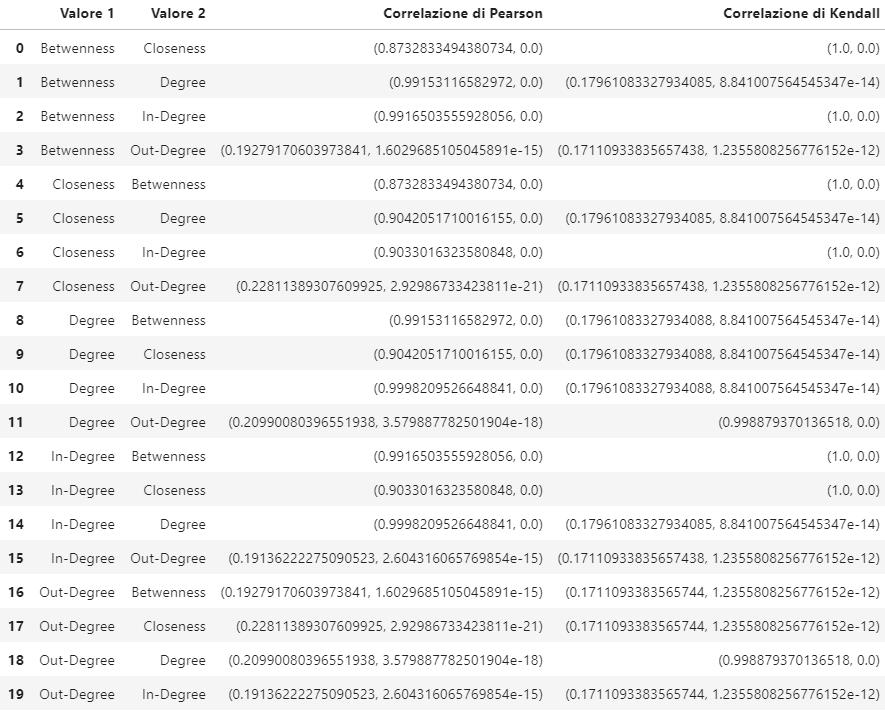
\includegraphics[width=0.9\linewidth]{tabella}
	\caption[Tabella della Correlazione di Pearson e Kendel relativa alle misure di centralità del grafo]{}
\end{figure}



\section{Conclusioni}
Dopo quest'analisi possiamo affermare che il grafo sociale costruito evidenzia la centralità dei nodi principali nel grafo, ma possiamo anche notare la presenza di nodi completamente scollegati da esso.\\
I risultati ottenuti dalle funzioni ci permette di affermare che il sottografo connesso si tratta di una rete \textbf{"Piccolo Mondo"}. \\
\pagebreak

\end{document}\\